\chapter{具有{S$_4$}对称性的外尔半金属}\label{chap:s4}

在破缺时间反演对称性但保持中心反演对称性的体系中,外尔点的出现可以由在八个中心反演不变点奇数条偶宇称/奇宇称占据态能带来保证。在这里,基于对称性分析和第一性原理计算,我们证明了对于有$S_4$的时间反演不变的体系,外尔半金属相可以由两个可以很好定义的不相等的不变量 $\eta$ 和$S_4$指标$z_2$来判断。
通过应用这个判据,我们发现一些之前认为是在非中心对称但有$S_4$对称性的空间群里发现的拓扑绝缘体的材料实际上是外尔半金属。
我们的第一性原理计算表明在有四对外尔点出现在$k_{x,y}$ = 0面,每个平面包含四个手性相同的外尔点。我们建立了有效模型来理解这些材料拓扑不平庸的本质。我们使用对称性指标和拓扑不变量的方法在对于时间反演不变的体系内寻找外尔半金属开辟了一条新的路径。 

\section{背景}
在过去的几十年,拓扑材料吸引了很多研究者的兴趣~\citep{bernevig2006quantum,zhang2009topological,Qi2010The,TIreview, Wan2011,wang2013three,Weng2016Topological,wang2016hourglass,PRBwzj,pre96wang,tqc2017,RevModPhys.90.015001,prb97wang}。许多拓扑绝缘体的候选材料首先被理论预言,后来又被实验证实~\citep{bernevig2006quantum, konig2007quantum, zhang2009topological, chen2009experimental, advwang}。大多数的预言都是通过拓扑不变量或者对称性指标来判断的~\citep{Fu2007topo, Fu2007IS,Slager2017, haruki2018, song2017, Vergniory2019, Zhang2018, wanxg2019}。拓扑外尔半金属~\citep{Murakami_2007,Liu2014Weyl,weng2015weyl,soluyanov2015type,lv2015observation,lv2015experimental,Weng2016Coexistence,PhysRevLett.117.236401,nie2017topological,sakai2018,prb99} 在具体的两重简并点附近有线性的色散。这个两重简并点被称为外尔点,它可以看作是动量空间贝利曲率的漏或源。他们表现出许多新奇的性质,比如在表面上的费米弧~\citep{Wan2011,xu2015discovery,xu2016observation,wang2016observation2},手性反常~\citep{huang2015observation,zhang2016signatures}, 和量子反常霍尔效应~\citep{Fang92,xu2011chern}等。但是,因为在三维空间外尔点不需要任何具体的对称性保护(除了平移对称性外),所以时间反演不变的(TRI)系统里的外尔半金属通常不能基于拓扑不变量和对称性指标来预测。据我们所知,对于时间反演对称性破缺(TRB)的中心对称体系,在中心反演不变的(ISI)动量上有奇数个偶/奇宇称占据态的能带可以保证外尔点的出现~\citep{Hughes2010Inversion,PhysRevLett.117.236401,nie2019magnetic}。这可以简单的通过两个平行的空间反演不变的平面上不等价的陈数(如果可以很好的定义)来简单的理解,如图~\ref{fig:5-1}(a) 和 \ref{fig:5-1}(b)所示。 在这里,我们的目的就是去找到可以保证外尔半金属相的合适的拓扑不变量或者定义在时间反演平面上的对称性指标。

\begin{figure}[!tb]
    \centering
    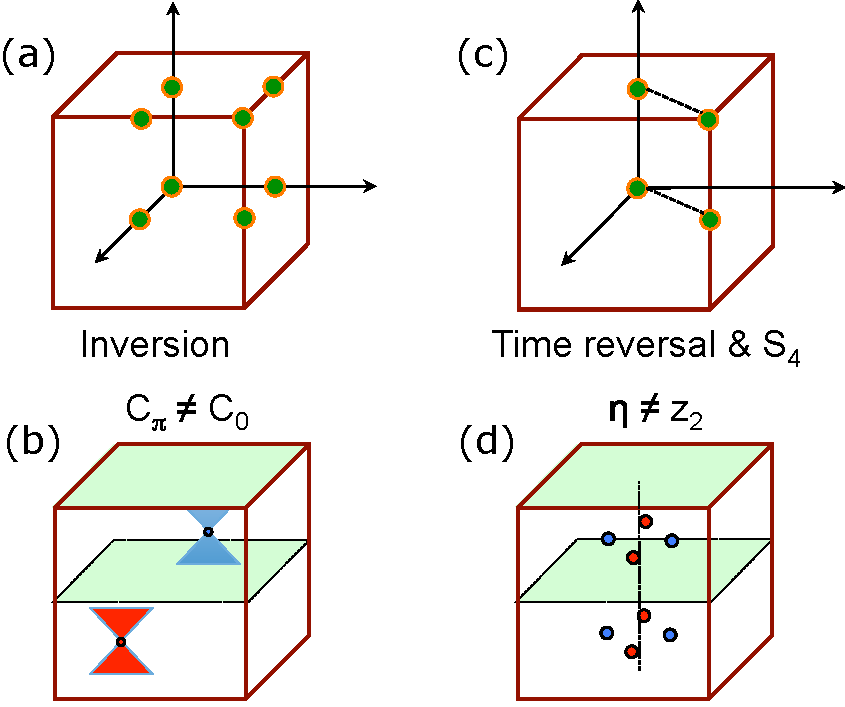
\includegraphics[width=9.2 cm]{s4-fig1.pdf}
    \bicaption{
        示意地展示具有对称指标和拓扑不变量的外尔半金属。
        对于时间反演对称性破缺的中心对称体系,在中心反演不变的动量 [(a)中绿色点 ] 上有奇数个偶/奇宇称占据态的能带,代表两个中心反演不变的平面的陈数是不同的(b),这可以保证3维布里渊区内有奇数对外尔点出现。注意,在时间反演不变的系统,偶/奇宇称占据态的能带数目总是偶数。对于具有时间反演不变和$S_4$对称性的系统,可以在四个$S_4$不变点[图(c)绿色点]的定义一个$z_2$指标,而且不变量$\eta$ [ 定义在正文内 ] 和$S_4~z_2$指标的不相等表明有外尔点出现,如图(d)。
        红色(蓝色)点代表+1(-1)手性的外尔点。~\citep{Qians4}
        } 
        {Schematic WSMs with symmetry indicators and topological invariants.
        For a TRB centrosymmetric system, an odd number of even/odd parity occupied bands at eight ISI momenta [green dots in (a)] reveals that the Chern numbers of the two ISI planes are different, which guarantee the appearance of odd pairs of Weyl points in 3D Brillouin zone (BZ) (b). Note that there is always an even number of even/odd parity occupied bands in a TRI system.
        For a TRI and $S_4$-symmetric system, a $z_2$ indicator is defined on four $S_4$ invariant momenta [green dots in (c)], and the inequality between the invariant $\eta$ [defined in the main text] and $S_4~z_2$ indicator reveals the appearance of Weyl points, as shown in (d). The red (blue) dots stand for +1 (-1) chiral Weyl points. ~\citep{Qians4}
    } 
    \label{fig:5-1}
\end{figure}

在这个工作中,我们主要关注有$S_4$对称性的时间反演不变的系统 (关于$S_4$不变的系统更一般的讨论可以参考文献~\citep{tobedone2019}) 。
在这些系统里,我们定义一个拓扑不变量$\eta$:
\begin{equation*}
(-1)^{\eta}=(-1)^{\nu_{a_1}}(-1)^{\nu_{a_2}},
\end{equation*}
只要有两个平行的完全开能隙的时间反演不变的平面(例如, $a_1$-面和$a_2$-面),这个不变量就可以很好的定义。不变量$\nu_{a_1}$ 和 $\nu_{a_2}$是两个平行的时间反演不变的平面内的时间反演不变的$\mathbb Z_2$不变量~\citep{Kane2005}。
此外,$ S_4 $对称性定义了对称性指示符$z_2$~\citep{song2017,haruki2018}。
注意,如果两个对称性指标都可以很好定义的话,在中心对称的时间反演不变的系统他们总是满足$\eta=z_2$~\citep{Fu2007topo,haruki2018}。这里,我们发现$\eta$ 和 $z_2$ 不相等意味着一般有外尔点出现(不考虑额外对称性)。具体来说,如果材料满足$\eta\neq z_2$则是外尔半金属,如图~\ref{fig:5-1} (b) 和~\ref{fig:5-1} (d) 。


%Fortunately, we find that it can be  the difference between three topological invariants [$\eta_i \equiv |{\mathbb Z}_{2,k_i=0}-{\mathbb Z}_{2,k_i=\pi}|,~i\in\{1,2,3\}$], where ${\mathbb Z}_{2,k_i=0(\pi)}$ is the TR $\mathbb Z_2$ invariant in the $k_i=0(\pi)$ plane and $k_{i=1,2,3}$ are along the directions of three primitive reciprocal lattice vectors. We note that the insulating phase has to satisfy the equivalence: $\eta_1=\eta_2=\eta_3$. It's also notable that a centrosymmetric system always satisfies the equivalence as long as the system is fully gapped.  Therefore, a system which does {\emph not} satisfy that equivalence can be a Weyl semimetal in general.  If we further consider S$_4$ symmetry, which defines another $\mathbb Z_2$ indicator ($z_2$), the equivalence that the insulating phase satisfies reduces to $\eta_z=z_2$.
许多年前,121号群 ($I\bar 42m$) 非中心对称的结构中的许多化合物被认为是拓扑绝缘体 ~\citep{Wang2010}。但是,我们仔细研究后发现,基于$S_4$对称性指标,这些所谓的“拓扑绝缘体”(``TIs")实际上可以分为两个不同的情况: $z_2=1$ (\tii~) 和 $z_2=0$ (\wsm~) 。
在这个工作,我们证明在\wsm~中的``TIs"实际上是外尔半金属。在$k_{x,y}=0$ 面上发现四对外尔点,每个平面包含四个手性相同的外尔点。此外,外尔点正好位于电荷中性能级。$\eta$ 和 $z_2$  (即, $\eta\neq z_2$) 可以来判别外尔半金属,这个方法也可以应用于其他具有$S_4$对称性的空间群~\citep{Haijun2016,HgTenc2016}。为了抓住121号空间群拓扑不平庸的物理本质,我们构造了六带低能有效模型。也给出了作为外尔半金属的标志的费米弧表面态。我们通过使用对称性指标和不变量找到外尔点的策略,开辟了一条在时间反演不变系统中搜索外尔半金属的新途径。


%We find that, in general, the Weyl semimetal phase with time-reversal symmetry is characterized by the difference between three topological invariants ($\eta_i \equiv |{\mathbb Z}_{2,k_i=0}-{\mathbb Z}_{2,k_i=\pi}|,~i\in\{1,2,3\}$), where ${\mathbb Z}_{2,k_i=0(\pi)}$ is the $\mathbb Z_2$ invariant in the $k_i=0(\pi)$ plane and $k_{i=1,2,3}$ are three primitive reciprocal lattice vectors.

%The difference between the $S_{4z}$ indicator ($\mathbb Z_{2,S_{4z}}$) of the two phases in these topological compounds intrigues us to investigate them further. These topological insulators have shared same TR $\mathbb Z_2$ invariants in the $k_z=0$ and $k_z=\pi$ planes: $\mathbb Z_{2,kz=0}=1$ and  $\mathbb Z_{2,kz=\pi}=0$, which is






\section{晶体结构和计算方法}
%Yuting,  Please fill it up with the description of crystal structures and Methodology.
%\emph{Crystal structure and Methodology.} -- 
{\it{晶体结构}}: 我们研究了锡矿结构中的一系列铜基硫族元素化物:Cu$_2$-Cu-Sb-VI$_4$ 和 Cu$_2$-II-IV-VI$_4$,其中 II=$\{$Cd, Hg, 和 Zn$\}$, IV=$\{$Si, Ge, 和 Sn$\}$, 和 VI=$\{$S, Se, 和 Te$\}$。这一系列化合物是空间群$I \bar 4 2 m$ ($D_{2d} $),体心四方结构,晶格常数为: $a$ 和 $c$。
% Among these compounds, we take Cu$_2$ZnGeSe$_4$ as an example for WSM and \ti for TI, respectively. More results on other compounds are presented in the Supplemental Material (SM).  Here we take Cu$_2$ZnGeSe$_4$ as an example .
这个结构有三个2度旋转轴($C_{2x,2y,2z}$), 两个镜面对称性 ($M_{xy,\bar xy}$),有时间反演对称 ($I$) 和四重旋转对称 ($C_{4z}$) 的组合对称操作 S$_4$,但是没有单独的 $I$ 和 $C_{4z}$。
在图~\ref{fig:5-2} (a) 展示了呈现锡矿结构。
每个阴离子均通过具有三个不等价键的四个阳离子进行四面体配位:VI-Cu,VI-II和VI-IV。
晶体结构沿$ c $轴几乎是二倍的闪锌矿结构,但由于层间耦合而具有以$c\neq2a$为特征的变形。这些化合物代表应变后的HgTe类材料~\citep{HgTenc2016}。

\begin{figure}[!tb]
\centering
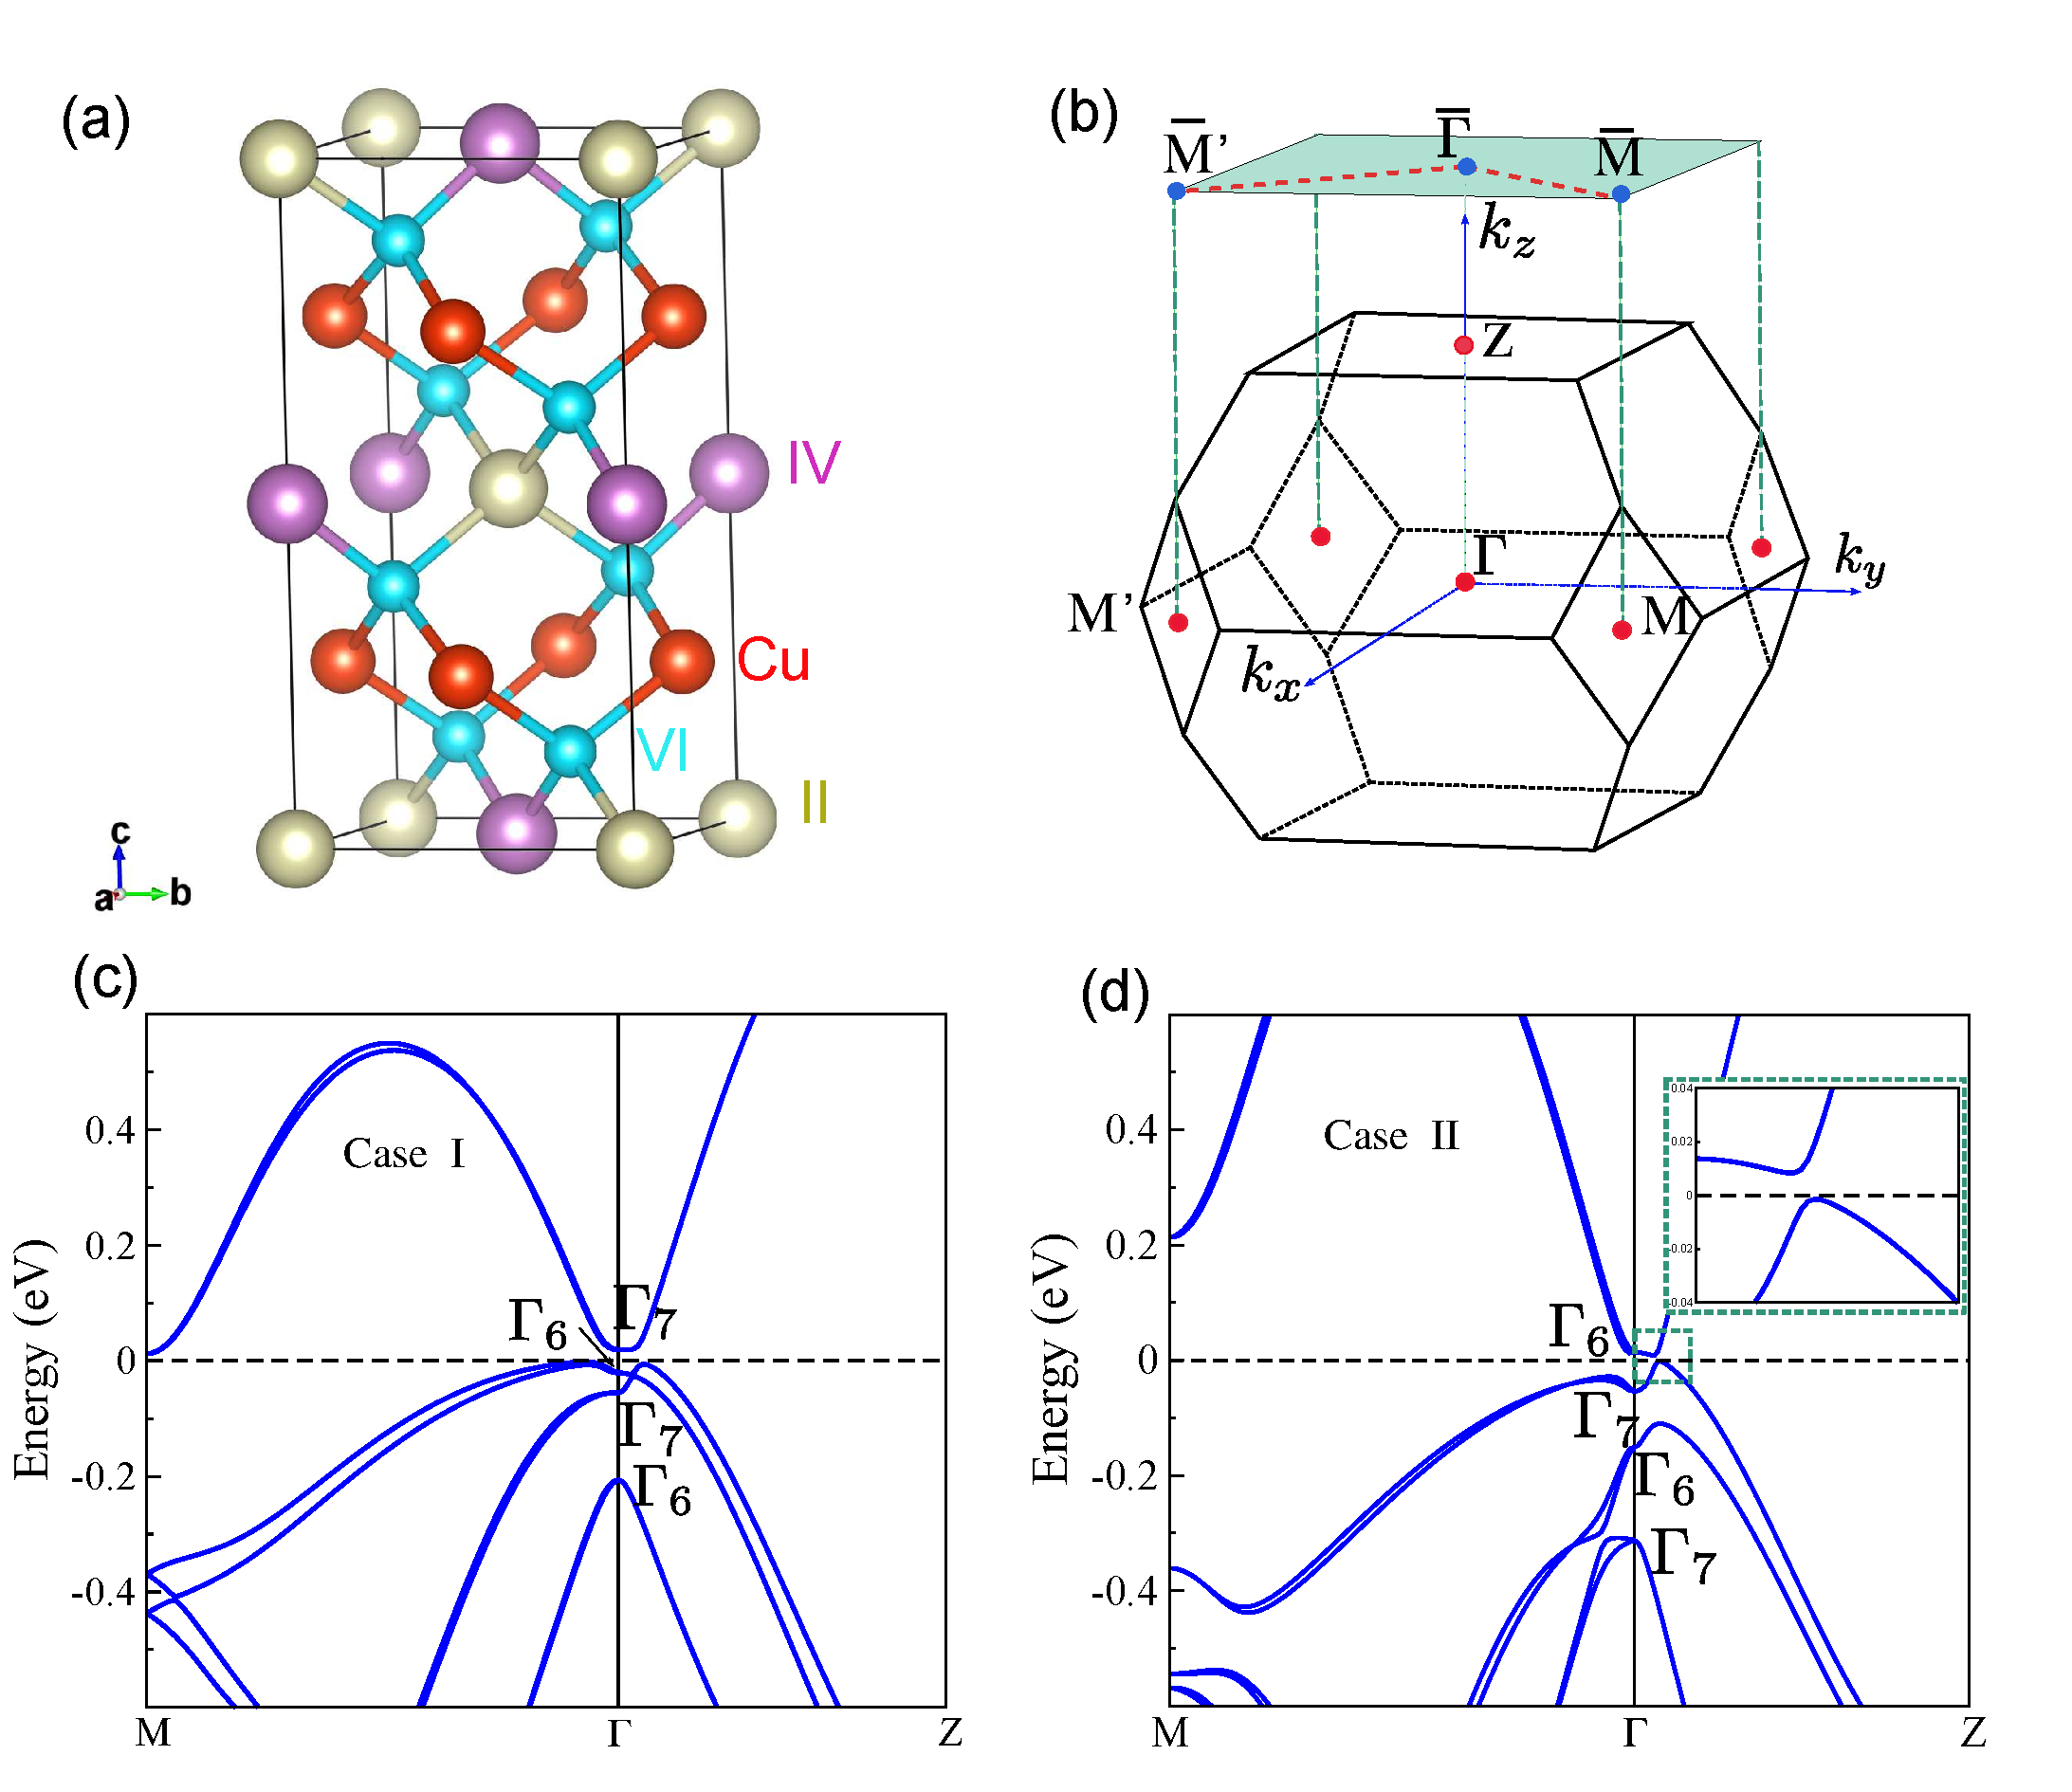
\includegraphics[width=8.5 cm]{s4-fig2.pdf}
\bicaption{
    (a)四元锡矿物Cu$_2$-II-IV-VI$_4$的晶体结构和(b)系列121空间群化合物的布里渊区。有混合的II和IV原子的交替阳离子层,它们通过Cu一价阳离子层相互分隔。两个等价的Cu原子, 一个II原子, 一个IV原子和四个VI原子分别占据$4d$, $2a$, $2b$ 和 $8i$ Wyckoff位置。在Cu$_2$-Cu-Sb-VI$_4$结构里, $2a$ 和 $2b$ 位置分别由Cu 和 Sb 原子占据。
    分别对\tii~和\wsm~给出了(c)\tic~和(d)\wsmc~的考虑SOC时的电子能带结构和$\Gamma$点的不可约表示。~\citep{Qians4}}
    {
    (a) Crystal structure of the quaternary stannite Cu$_2$-II-IV-VI$_4$ compounds and (b) BZ for the series of compounds in space group 121. There are alternating cation layers of mixed II and IV atoms, which are separated from each other by layers of Cu monovalent cations. Two equivalent Cu atoms, one II atom, one IV atom and four VI atoms occupy the $4d$, $2a$, $2b$ and $8i$ Wyckoff positions, respectively. In the Cu$_2$-Cu-Sb-VI$_4$ structure, the $2a$ and $2b$ positions are occupied by Cu and Sb atoms, respectively.
    The electronic band structures and irreps at $\Gamma$ point with SOC for (c) \tic~and (d) \wsmc~are presented for \tii~ and \wsm, respectively. ~\citep{Qians4}
    } \label{fig:5-2}
\end{figure}


{\it{计算方法}}: 
我们使用基于密度泛函理论的缀加平面波方法\citep{paw1,paw2}的VASP软件包\citep{KRESSE199615,vasp}进行第一性原理计算。
 %were employed in our first-principles calculations.
 交换关联泛函选取GGA的PBE泛函~\citep{pbe}。平面波的动能截断为400 eV。自洽计算过程对布里渊区取样为10$\times$10 $\times$10 $k$网格。晶体结构和原子参数来自Inorganic Crystal Structure Database (ICSD),展示在表格~\ref{tab:5-s1}。计算了考虑自旋轨道耦合(SOC)的电子能带结构。采用Wilson-loop方法~\citep{Yu2011An}计算拓扑不变量和手性电荷~\citep{Fang92}。


\section{结果和讨论}
\subsection{电子能带结构}
\begin{figure*}[!htb]
    \centering
    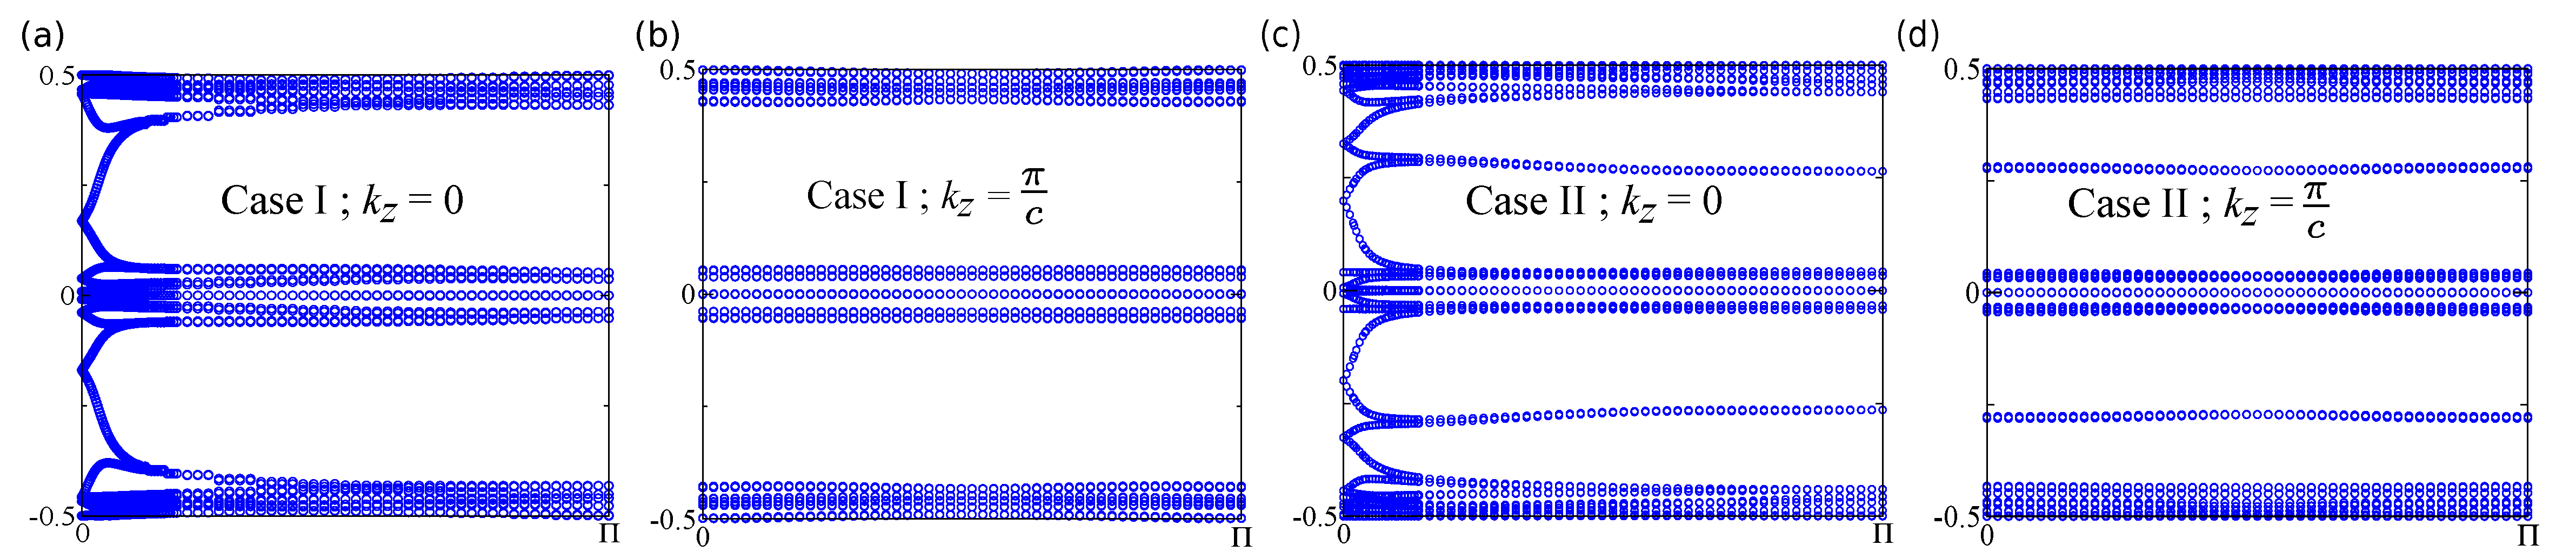
\includegraphics[height=3.2cm]{s4-fig4z2.pdf}
    \bicaption{
    (a, b)和(c, d)分别为\tii~和\wsm~在$k_z=0$ 和 $k_z={\frac{\pi}{c}}$平面上时间反演$\mathbb Z_2$的计算结果。~\citep{Qians4}
    }{
    The calculated time-reversal $\mathbb Z_2$ in  $k_z=0$ and $k_z={\frac{\pi}{c}}$ planes for \tii~ (a, b) and \wsm~ (c, d), respectively. ~\citep{Qians4}
    } \label{fig:5-s2}
    \end{figure*}
    
基于第一性原理计算,我们对先前工作中认为拓扑绝缘体的一类材料的能带结构重新进行了研究~\citep{Wang2010}。
我们发现这些化合物其实可以分为两类。在文章中,我们将\tic~(\tii) 和 \wsmc~(\wsm) 化合物分别作为这两种情况的例子,沿着高对称线上计算得到的能带结构如图~\ref{fig:5-2}。其他化合物的能带结果如图~\ref{fig:5-s1},这里使用的是ICSD报道的实验的晶格常数[如表~\ref{tab:5-s1}].
%qianyt
%For the series of the compounds in space group 121, we have systematically computed band structures and time-reversal $\mathbb Z_2$ invariants in the two planes: $k_z=0$ and $k_z=\frac{\pi}{c}$ as shown in Fig.~\ref{fig:5-s1} and Fig.~\ref{fig:5-s2}, respectively. The experimental parameters are employed as reported in the ICSD [shown in Table~\ref{tab:s1}]. We present the band structures of the topological compounds with $\eta=1$. For all these topological compounds, $\nu_{k_z=0}=1$ and $\nu_{k_z=\frac{\pi}{c}}=0$ are in the two planes, respectively. These topological compounds are previously predicted to be TIs~\citep{Wang2010}. However, after we determine the irreps of the low-energy bands~\citep{Gao2020}, one can easily find that they can actually be classified into two cases: \tii~has the $\Gamma_7$ band as the LCB (the upper panels of Fig.~\ref{fig:5-s1}), while \wsm~has the $\Gamma_6$ band as the LCB (the lower panels of Fig.~\ref{fig:5-s1}). In the following discussion, we show that the two cases actually correspond to different values of the $S_4~z_2$ indicator.


\begin{figure*}[!htb]
\centering
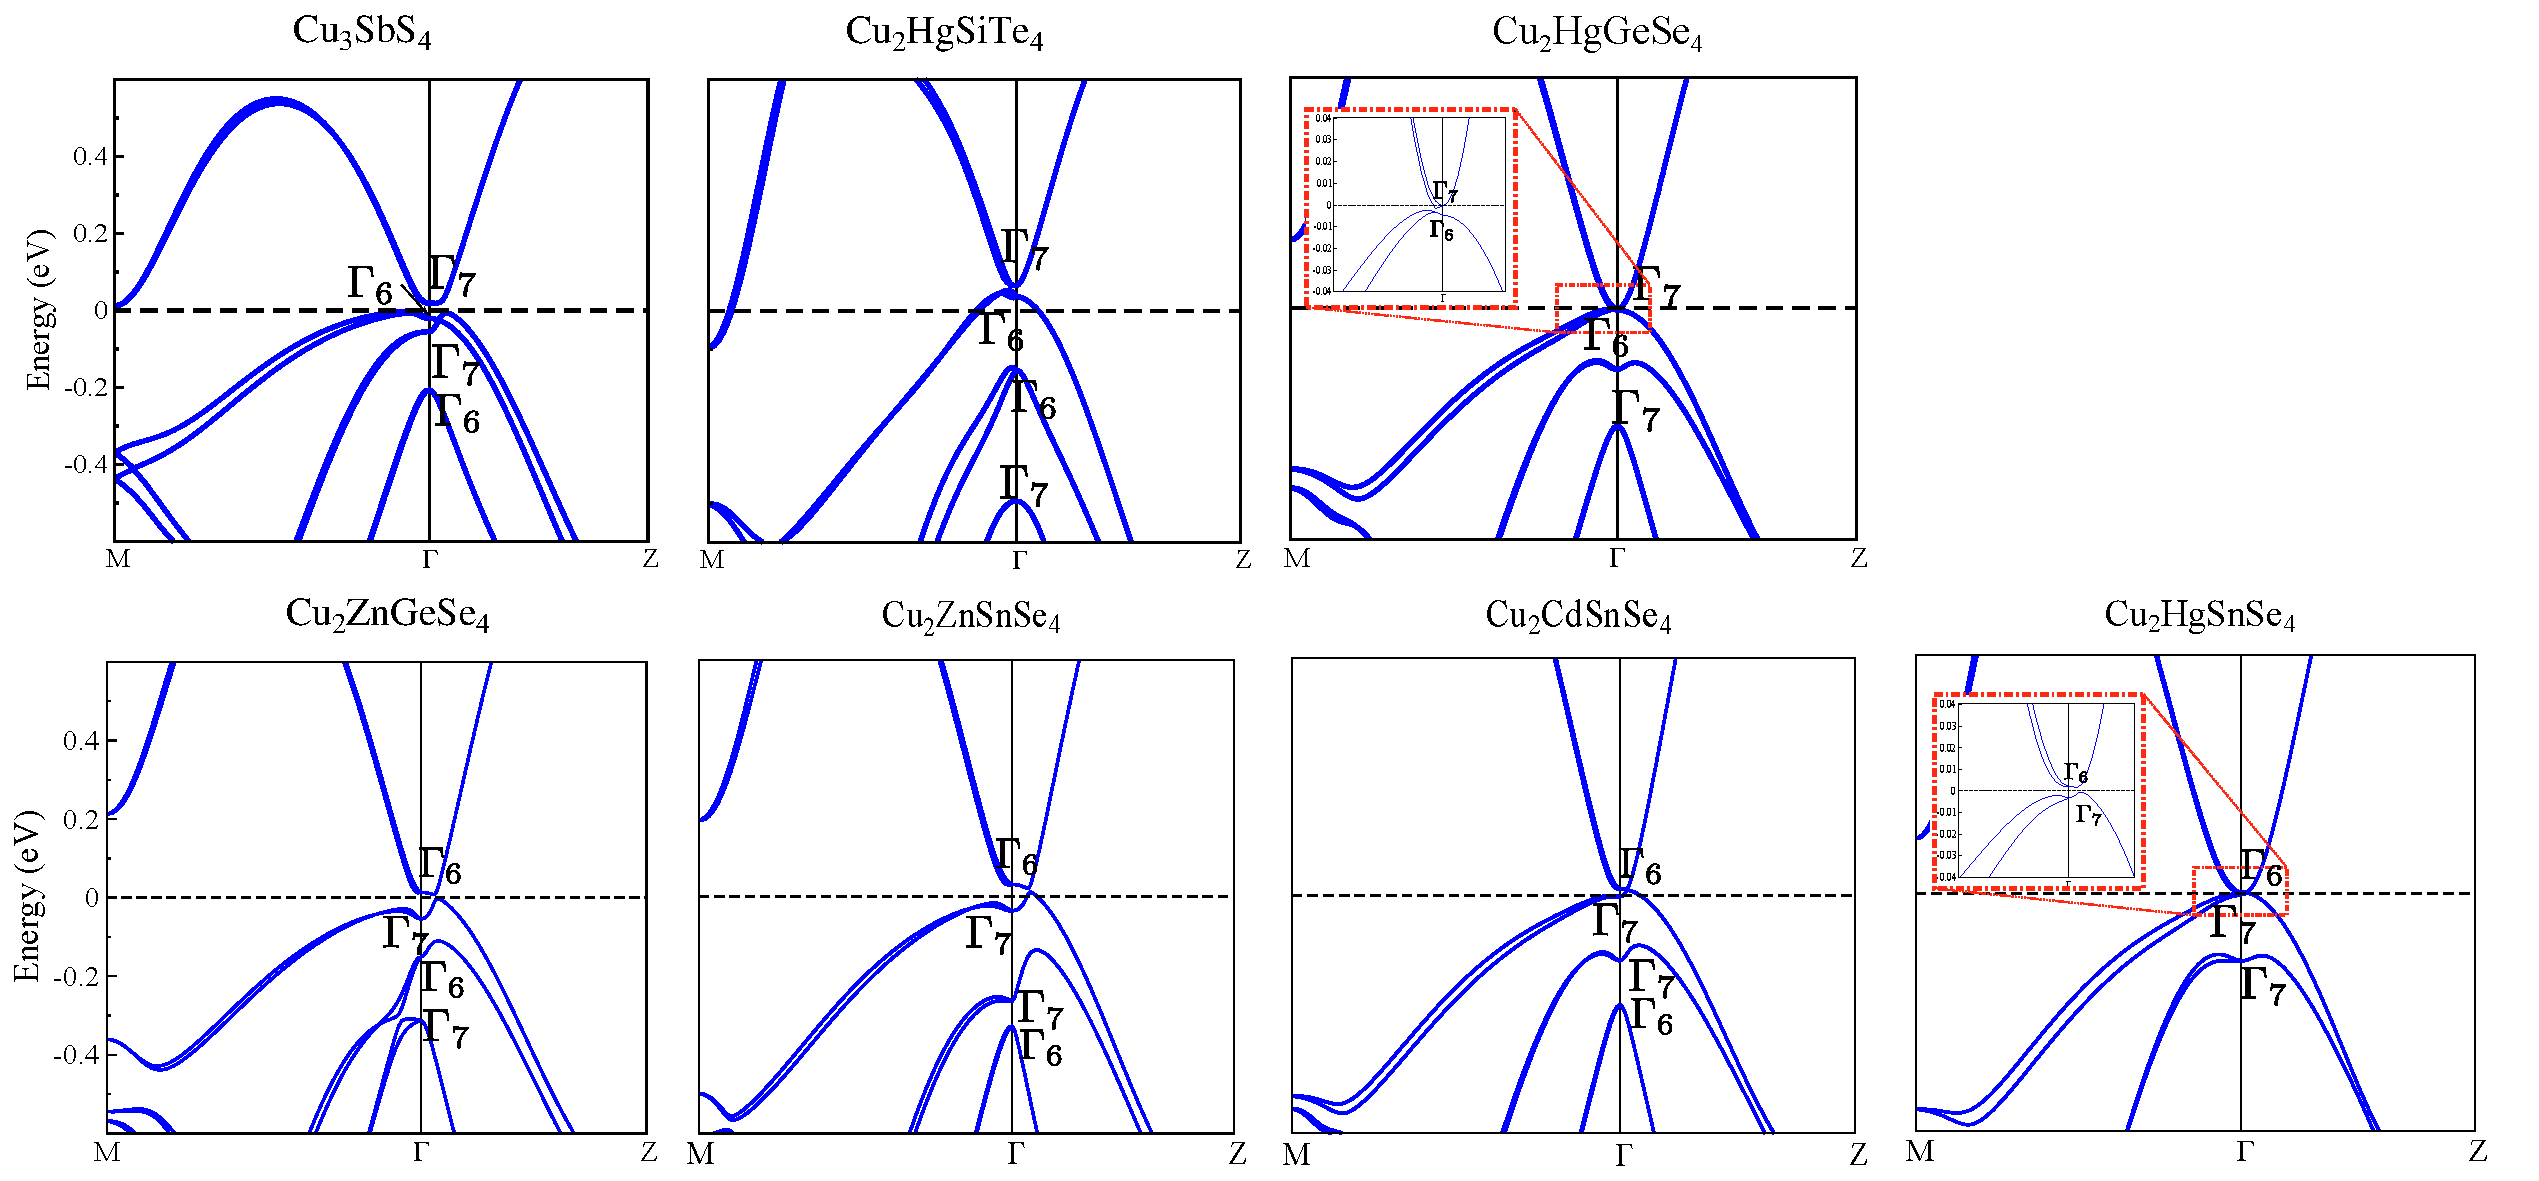
\includegraphics[height=7cm]{s4-figsband.pdf}
\bicaption{
考虑SOC时,这些有$\eta=1$的拓扑材料的能带结构和$\Gamma$点的能带表示。具体地,这些化合物在$k_z=0$面上有非平庸的$\mathbb Z_2$不变量, 但在 $k_z=\frac{\pi}{c}$的面有平庸的$\mathbb Z_2$不变量。~\citep{Qians4}
}
{
The electronic energy bands with SOC and band irreps at the $\Gamma$ point of topological compounds with $\eta=1$. Explicitly, these compounds have a nontrivial $\mathbb Z_2$ invariant in the $k_z=0$ plane, but a trivial $\mathbb Z_2$ invariant in the $k_z=\frac{\pi}{c}$ plane. ~\citep{Qians4}
}
\label{fig:5-s1}
\end{figure*}


\begin{table}[!htb]
    \bicaption{
        考虑SOC时,具有拓扑的化合物的ICSD编号和拓扑分类。~\citep{Qians4}
    }{
     ICSD numbers and topological classifications for these topological compounds with SOC. ~\citep{Qians4}
    }\label{tab:5-s1}
    \centering
    \resizebox{\textwidth}{!}{
    \begin{tabular}{cccc}
    \cline{1-4}
    \cline{1-4}
    \cline{1-4}
    Compound &ICSD Num. &Previous& This work[units: ($\frac{2\pi}{a},\frac{2\pi}{a},\frac{2\pi}{c}$)]\\
    \cline{1-4}
    Cu$_3$SbS$_4$ &  628824\citep{Annamamedov1967}& TI\citep{Wang2010} &TI    \\
    Cu$_2$HgSiTe$_4$ &656152\citep{Haeuseler1991} &TI\citep{tqc2017,Vergniory2019}&TI  \\
     Cu$_2$HgGeSe$_4$ & 627692\citep{Hahn1965}&TI\citep{Wang2010}&TI \\
    Cu$_2$HgGeTe$_4$ & 656155\citep{Haeuseler1991}&TI\citep{tqc2017,Vergniory2019}&TI  \\
    Cu$_3$SbSe$_4$ &  628997\citep{Annamamedov1967}& TI\citep{tqc2017,Vergniory2019}&TI  \\
%    \cline{1-4}
    %Compound &ICSD Num. & Previous& This work [units: ($\frac{2\pi}{a},\frac{2\pi}{a},\frac{2\pi}{c}$)]
    Cu$_2$ZnGeSe$_4$ &627831\citep{Guen1979}&TI\citep{Wang2010}& WSM (0.0036, 0.0, 0.0657)\\
    Cu$_2$ZnSnSe$_4$ &629099\citep{Hahn1965}&TI\citep{Wang2010}& WSM (0.0037, 0.0, 0.0757)\\
    Cu$_2$CdSnSe$_4$ &619784\citep{Hahn1965}& TI\citep{Wang2010}&WSM (0.0014, 0.0,  0.0294)\\
    Cu$_2$HgSnSe$_4$ &627936\citep{Hahn1965}&TI\citep{Wang2010}& WSM (0.0049,  0.0,  0.0238)\\
    Cu$_2$HgSnTe$_4$ &627940\citep{Haeuseler1991}&Trivial\citep{tqc2017,Vergniory2019}& WSM (0.0082,  0.0,  0.0338)\\
    %                         &&  && &Cu$_2$HgSnTe$_4$ &656158\citep{Haeuseler1991}& Trivial\citep{Zhang2018}&WSM (0.0066, 0.0,   0.0191)\\
    \cline{1-4}
    \cline{1-4}
    \cline{1-4}
    \end{tabular}}
    \end{table}
%We find that the band these compounds can he others are qualitatively identical to these two compounds [see more results of other topological candidates in the SM].
%Without loss of generality, we take two examples of \ti~and \wsm~compounds in the main text. The others are qualitatively identical to these two compounds [see more results of other topological candidates in the SM].
我们发现这两种化合物沿着高对称线都有一个带隙。然后,我们计算了$k_z=0$ 和 $k_z=\frac{\pi}{c}$平面上的时间反演不变的$\mathbb Z_2$不变量。 
Wilson loop的计算结果如图~\ref{fig:5-s2}。
%The results of the Wilson loop calculations are presented in Fig.~\ref{fig:5-s2} of Appendix A.
两个$\mathbb Z_2$不变量计算结果为$\nu_{k_z=0}=1$ 和$\nu_{k_z=\frac{\pi}{c}}=0$, 使得$\eta=1$ (或者 $\nu_0=1$ 如果系统在三维布里渊区里完全是开能隙的~\citep{Fu2007topo}) 。这些结果与之前预测的``TIs"的结果是一致的 \citep{Wang2010}。 在本文中,``TIs"代表那些之前预测的121号空间群中$\eta=1$的拓扑材料。

然后,我们进一步检查了电子态的不可约表示~\citep{Gao2020}。在Case I, $\Gamma$点上最低的导带表示是$\Gamma_7$ ,而对于\wsm~最低导带表示是$\Gamma_6$。
$\Gamma_6$ 和 $\Gamma_7$是$\Gamma$点的小群( $D_{2d}$双群)表示的标记。
%%appendix
因为在考虑自旋的体系内 $S_4^4=-1$, $S_4$的本征值为 $\lambda_j=e^{i\pi\frac{2j-1}{4}}$, 其中 $j\in\{0,1,2,3\}$。在具有$S_4$对称性的时间反演不变的体系中,我们提出$S_4$的$z_2$指标的一个一般的定义:
\begin{equation}
  z_2 = \sum_{K\in\{\text{four SIM}\}}\frac{n_K^{2} - n_K^{0}}{2} \quad{\rm mod} \ 2 ,
\end{equation}
这里 $n_K^{i}$ 为在$S_4$不变的动量(SIM)$K$点,有$S_4$ 本征值 $\lambda_i$的占据态能带的数目,细节推导参考文献~\cite{tobedone2019}。
如果这四个SIM也是时间反演不变点(TRIM),那么这个定义与文献~\citep{song2017,haruki2018} 的定义是一致的。

\begin{figure}[!htb]
\centering
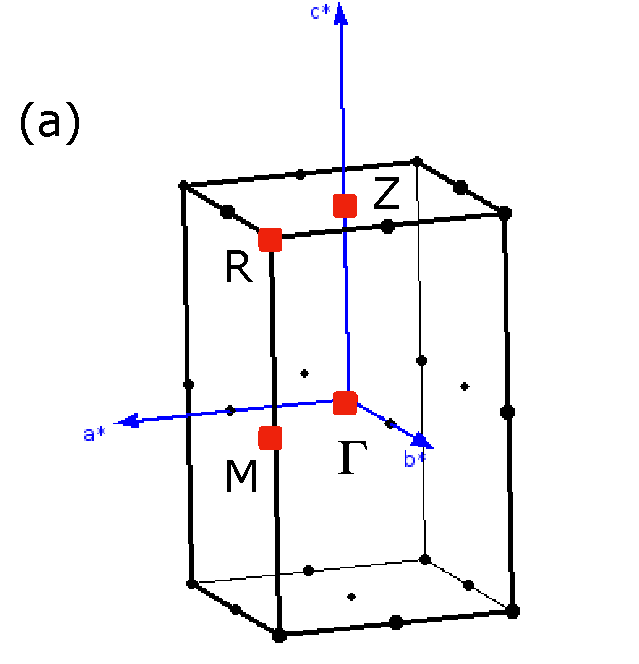
\includegraphics[width=2.5 cm]{s4-scbz.pdf}
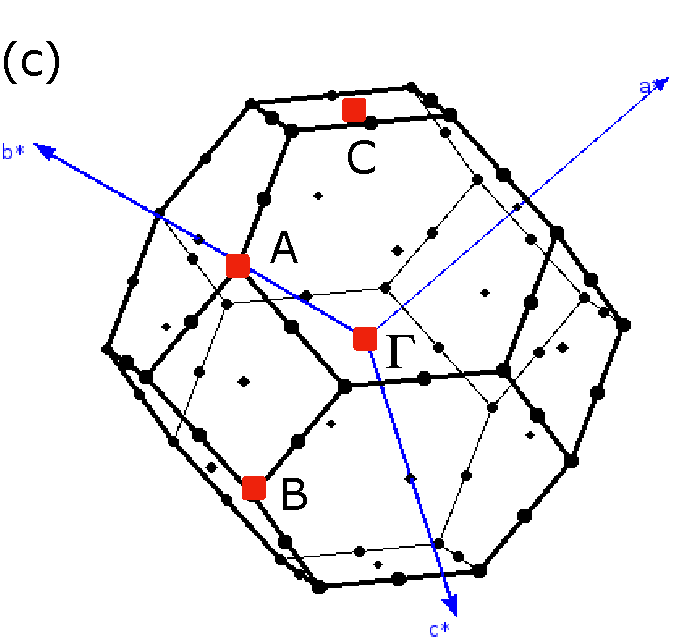
\includegraphics[width=2.5 cm]{s4-fccbz.pdf}
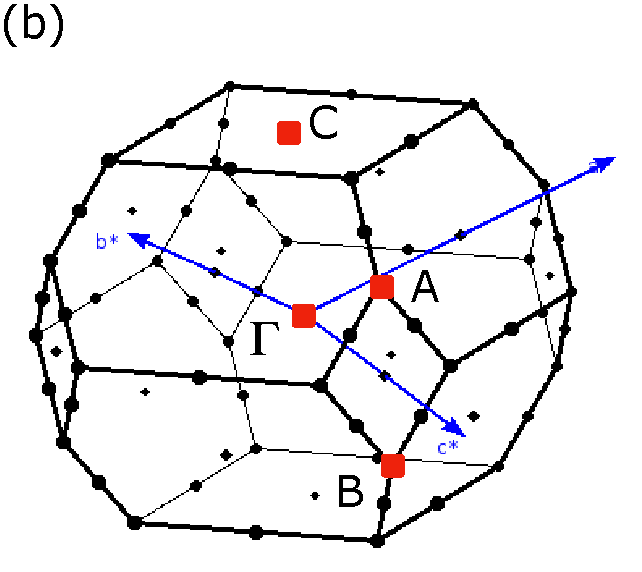
\includegraphics[width=2.5 cm]{s4-bccbz.pdf}
\bicaption{
三维布里渊区和SIM点。我们分别展示了简单晶格(a),面心晶格(b),体心晶格(c)的三维布里渊区。SIM点也在图中标记出来。~\citep{Qians4}
}
{
The 3D BZs and SIM points. We present the 3D BZs for simple lattice (a), and face-centered lattice (b),and body-centered lattice (c)  respectively. The SIM points are labeled too. ~\citep{Qians4}
}
\label{fig:5-bz}
\end{figure}

%\subsubsection*{a. Space group $P{\bar 4}$ (\#81)}
在简单四方结构(SG 81 和它的母群)如图\ref{fig:5-bz} (a) , 四个SIM为$\Gamma[0,0,0]$, $Z[0,0,0.5]$, $M[0.5,0.5,0.0]$, 和 $R[0.5,0.5,0.5]$ (此后,所有$k$点都是以[$\frac{2\pi}{a},\frac{2\pi}{a},\frac{2\pi}{c}$]为单位的笛卡尔坐标)。因为四个SIM也是时间反演不变点,所有点能带都是两重简并的。因此,$n_K^{\frac{1}{2}}~(n_K^{\frac{3}{2}})$ 等于 $n_K^{0}~(n_K^{2})$。
按照文献~\citep{song2017,haruki2018}的定义, $n_K^{\frac{1}{2}}~(n_K^{\frac{3}{2}})$ 是在$K$点满足tr$[D(S_4)]=\sqrt{2}$(tr$[D(S_4)]=-\sqrt{2}$)的Kramers对的数目, 其中$D(S_4)$ 是相应的Kramers对的表示矩阵。
\begin{equation}
  z_2 = \sum_{K\in\{\Gamma,Z,M,R\}}\frac{n_K^{\frac{3}{2}} - n_K^{\frac{1}{2}}}{2} \quad{\rm mod} \ 2 ,
\end{equation}

在面心立方结构(SG 216 和它的母群)如图\ref{fig:5-bz}(b), 四个 SIM是 $\Gamma[0,0,0]$, $C[0,0,1]$, $A[1,0,0.5]$, 和 $B[1,0,-0.5]$。 $A$ 和 $B$ 不是TRIM,没有Kramers简并。因此 $S_4$ $z_2$ 指标定义为,
\begin{equation}
  z_2 = \sum_{K\in\{\Gamma,C,A,B\}}\frac{n_K^{2} - n_K^{0}}{2} \quad{\rm mod} \ 2 ,
\end{equation}

在体心四方结构 (SG 82 和它的母群)如图\ref{fig:5-bz}(c), 四个SIM为$\Gamma[0,0,0]$, $C[0,0,1]$, $A[0.5,0.5,0.5]$, 和 $B[0.5,0.5,-0.5]$。注意到$A$ 和 $B$ 不是TRIM。换句话说,在$A$ 和 $B$点没有Kramers对。所以,$S_4$ $z_2$ 指标的定义为,
\begin{equation}
  z_2 = \sum_{K\in\{\Gamma,C,A,B\}}\frac{n_K^{2} - n_K^{0}}{2} \quad{\rm mod} \ 2 ,
\end{equation}
因为121号群有体心四方结构, 四个SIM的$n_K^{0}$ 和 $n_K^{2}$具体的计算结果在表格~\ref{tab:5-weyls4}给出。
这个$z_{2}$ 指标对于\tii~和\wsm~的计算结果分别为1和0 [参考表格~\ref{tab:5-weyls4}]。

%{\color{blue}NOTE: PLEASE CHANGE ALL S4 $\mathbb Z_2$ to $z_2$.}
\begin{table}[!h]
    \centering
    \caption{
    占据态在SIM点有$S_4$本征值$\lambda_2$和 $\lambda_0$的数目。最后一列展示了计算得到的$S_4$ $z_2$指标。~\citep{Qians4}
      }
      {
    The number of occupied states with $S_4$ eigenvalue $\lambda_2$ and $\lambda_0$ at SIM. The last column shows the determined $S_4$ $z_2$ indicator. ~\citep{Qians4}
      }\label{tab:5-weyls4}
      \begin{tabular}{cccccc}
      \hline
      $n_K^{2},n_K^{0}$ & $\Gamma$ & C & A & B & $S_4~z_2$  \\
      \hline
       \tii~(TI)   & 15,16 & 16,15 & 16,15 & 16,15 & 1 \\
       \wsm~(WSM) & 14,17 & 16,15 & 15,16 & 15,16 & 0 \\
      \hline
      \end{tabular}
\end{table}
    

在三维绝缘相, 强拓扑绝缘体(STI)指标 $\nu_0$~\citep{Fu2007topo} 定义在八个不同的时间反演不变的动量上 [$\Gamma_{i=(n_1n_2n_3)}=(n_1 \bb_1+n_2 \bb_2+n_3\bb_3)/2$, 其中 $n_j=0,1$,$b_j$是倒空间原胞基矢] : 
\begin{equation*}
(-1)^{\nu_0}=\prod_{n_j=0,1}  \delta_{n_1n_2n_3}=(-1)^{\nu_{a_1}}(-1)^{\nu_{a_2}},
\end{equation*}
这里 $\delta_i=\sqrt{det[w(\Gamma_i)]}/Pf[w(\Gamma_i)]$ 其中幺正矩阵 $w_{ij}(\bk)=\braket{u_i(\bk)}{{\cal T}|u_j(\bk)}$。 这里 $\ket{u_j(\bk)}$ 布洛赫函数的周期部分。在 $\bk=\Gamma_i$, $w_{ij} =-w_{ji}$, 所以 Pfaffian $Pf[w(\Gamma_i)]$ 有好的定义。
因为四个$\delta_i$的定义了二维时间反演不变的平面的$\mathbb Z_2$(如果四个$\Gamma_i$形成一个平面),
强拓扑绝缘体对称性指标$\nu_0$也可以通过两个平行平面($a_1$- 面和$a_2$- 面) 的两个不同的$\mathbb Z_2$不变量来定义($\nu_{a_1}$ and $\nu_{a_2}$)来定义, 当$\eta=\nu_0$产生绝缘体。注意,如果三维体态完全开能隙,$\nu_0$可以很好的定义;而只要存在两个完全开能隙的时间反演不变的平面,$\eta$就有好的定义。另一方面,当有额外的$S_4$对称性, 对于绝缘体,$S_4$的$z_2$指标和强拓扑绝缘体的指标$\nu_0$是一致的~\citep{song2017,haruki2018}。
因此,121号空间群的``TIs"中,有平庸的$z_2$指标的\wsm~不是绝缘体。最终,我们发现这些候选材料其实是外尔半金属,有四对外尔点在电荷中性能级。

%%qianyt
因为PBE函数计算得到的能隙一般会被低估,为了检查121号群这些外尔半金属相 (参考表格~\ref{tab:5-s1})能带反转的稳定性,我们使用修正的Becke-Johnson(mBJ)势进行了更精确的计算。由于这些材料能带结构的主要特点是在$\Gamma$点能带的顺序,我们系统的检查了在$\Gamma$点的四条能带(三条价带和一条导带),并将其作为mBJ 参数的($C_\text{mBJ}$) 函数展示在图~\ref{fig:5-mbj}中。对于\tii~的能量顺序为$\Gamma_7$, $\Gamma_6$ 和 $\Gamma_7$ (从高能到低能), 而对于\wsm~是$\Gamma_6$, $\Gamma_7$ 和 $\Gamma_7$ 。随着C$_{\text{mBJ}}$的减小,我们可以清楚的看到表示为 $\Gamma_6$的导带的能量单值减小。相应地,$\Gamma_6$的导带和三条价带相交,两个$\Gamma_6$表示的能带不能相交。在图~\ref{fig:5-mbj}中,C$_{\text{mBJ}}$的临界值用虚线表明,代表$\Gamma_6$的导带与其他更高的价带发生能带反转的地方。
结果表明Cu$_2$HgGeTe$_4$, Cu$_3$SbSe$_4$, Cu$_2$HgSnSe$_4$, 和  Cu$_2$HgSnTe$_4$ 的C$_{\text{mBJ}}$比较大,大概是1.2,所以这些化合物能带反转比较可信。
其中, Cu$_2$HgSnTe$_4$非常有可能是外尔半金属的候选材料,因为能带反转发生在比较大的mBJ参数$C_\text{mBJ}=1.25$。最近的实验\citep{PhysRevB.100.195147}已经通过STM和ARPES中发现Cu$_2$HgSnSe$_4$的半金属的特点。
 


\begin{figure*}[!htbp]
    \centering
    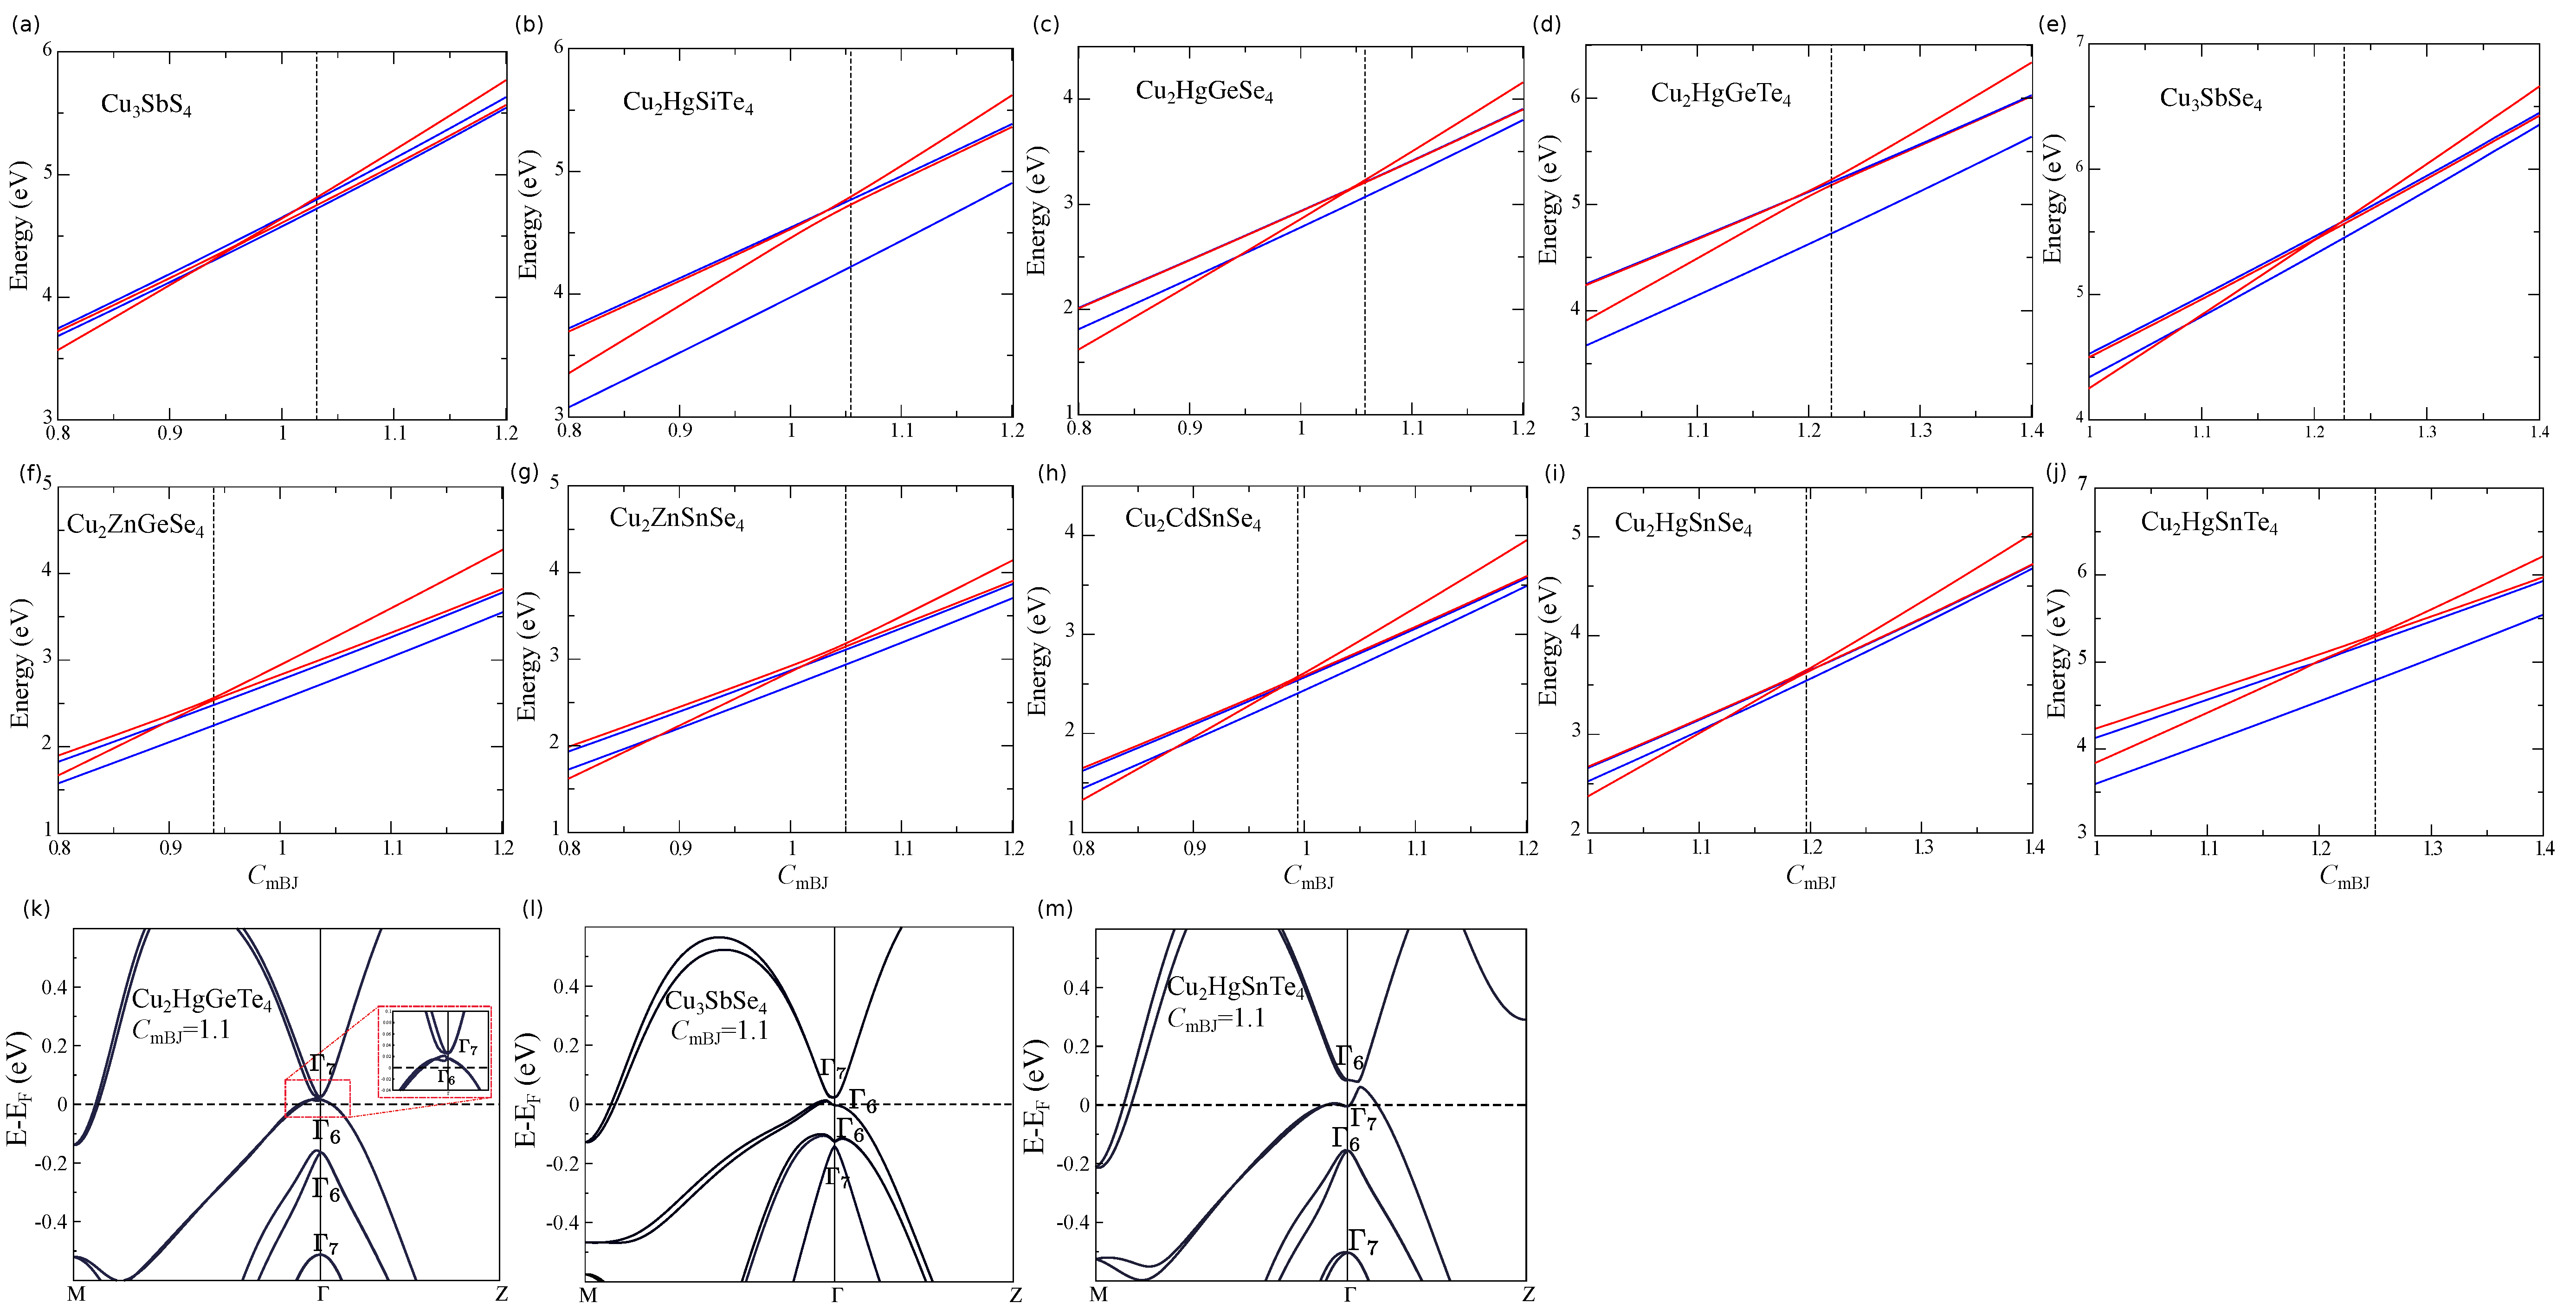
\includegraphics[height=7.5cm]{s4-cmbj.pdf}
    \bicaption{(a-j)展示了不同化合物$\Gamma$处费米能级附近四条能带(三条价带和一条导带)随着$C_\text{mBJ}$ 的演化。表示为$\Gamma_6$和$\Gamma_7$ 的能带分别用红色和蓝色线表示。
    (k-m)代表考虑SOC且$C_\text{mBJ}=1.1$时Cu$_2$HgGeTe$_4$(k), Cu$_3$SbSe$_4$(l), and Cu$_2$HgSnTe$_4$的能带结构。~\citep{Qians4}
    }
    {(a-j) show the band evolutions of four bands near the Fermi level (three valence bands and one conduction band) at the $\Gamma$ point with varying the parameter $C_\text{mBJ}$ for different topological compounds.  The $\Gamma_6$ and $\Gamma_7$ bands are denoted by the red and blue lines, respectively.
    (k-m) present the SOC electronic structures with $C_\text{mBJ}=1.1$ for Cu$_2$HgGeTe$_4$ (k), Cu$_3$SbSe$_4$ (l), and Cu$_2$HgSnTe$_4$ (m), respectively. ~\citep{Qians4}
    }
    \label{fig:5-mbj}
\end{figure*}


\subsection{外尔点和Wilson loop计算}

\begin{figure*}[!htb]
    \centering
    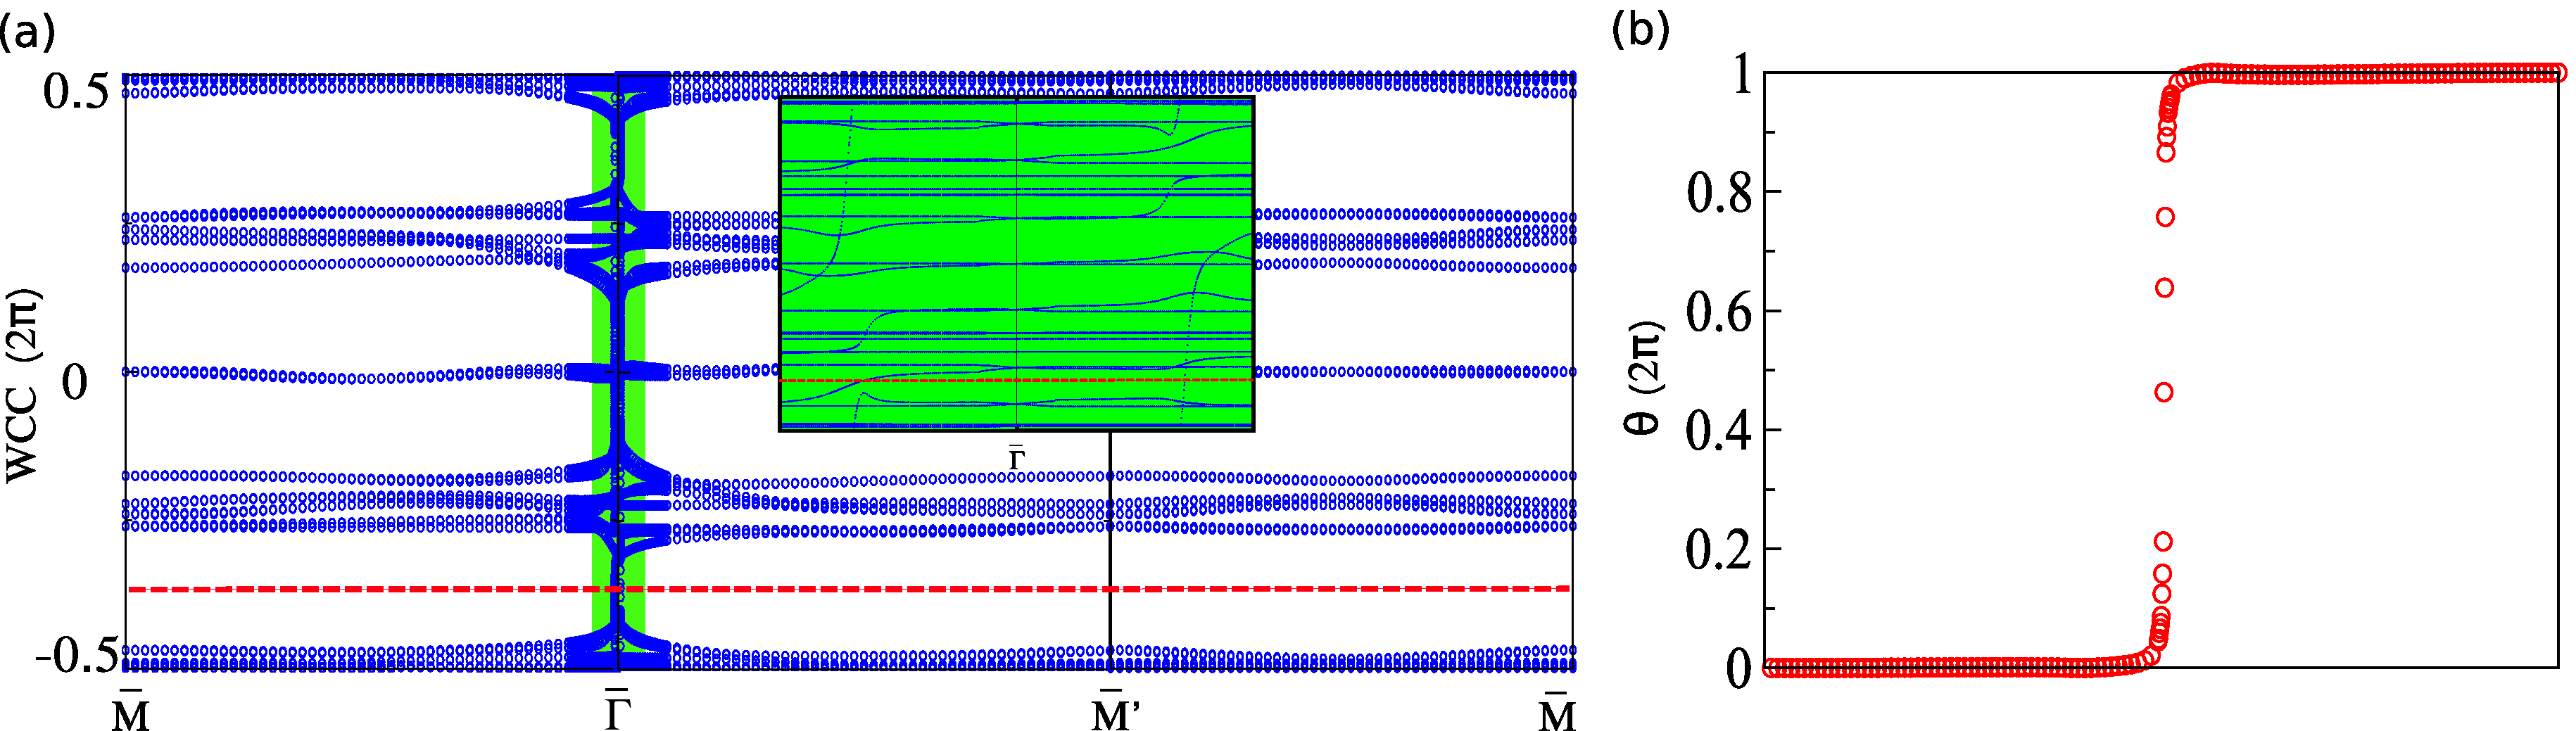
\includegraphics[width=1\textwidth]{s4-fig3.pdf}
    \bicaption{
        (a)\wsmc~沿着路径$\bar M (0.5,0.5)-\bar \Gamma(0,0)-\bar M'(0.5,-0.5)-\bar M(0.5,0.5)$(如图~\ref{fig:5-2})的$k_z$-指向的Wilson loops的WCC。(b) 在包裹外尔点的流形上通过Wilson-loop方法计算的位于[ $0.0036(\frac{2\pi}{a}), 0.0, 0.0657(\frac{2\pi}{c}$) ]的外尔点的手性。~\citep{Qians4}
        }
        {
        (a) The WCC of $k_z$-directed Wilson loops of \wsmc~on the path $\bar M (0.5,0.5)-\bar \Gamma(0,0)-\bar M'(0.5,-0.5)-\bar M(0.5,0.5)$ as marked in Fig.~\ref{fig:5-2}. (b) The chirality of the Weyl point at [$0.0036(\frac{2\pi}{a}), 0.0, 0.0657(\frac{2\pi}{c}$)] calculated by Wilson-loop method on a manifold enclosing it. ~\citep{Qians4}
    } 
    \label{fig:5-3}
    \end{figure*}
%\emph{Weyl points and Wilson loop calculations.} -- 
为了确定外尔点的位置,我们计算了在$k_xk_y$平面,WSM \wsmc~沿着路径: $\bar M [0.5,0.5]-\bar \Gamma[0,0]-\bar M'[0.5,-0.5]-\bar M[0.5,0.5]$(以$[\frac{2\pi}{a},\frac{2\pi}{a}]$为单位 )$k_z$-指向的Wilson loops。如图~\ref{fig:5-3}(a),结果显示有非零的陈数$C=+2$, 这意味着由面内的路径和$k_z$轴构成的二维闭合的流形至少包围有两个手性为+1的外尔点~\citep{Fang92}。
首先, 我们假设在流形的一般位置[$x_1 (\frac{2\pi}{a}),y_1 (\frac{2\pi}{a}),z_1 (\frac{2\pi}{c})$]上有一个手性为+1的外尔点。因为在$k_z=0$面完全打开能隙,$z_1$ 应该是非零的(即,$z_1\neq 0$)。
然后,组合对称性${\cal T}C_{2z}$得出在[$x_1,y_1,-z_1$]位置也有一个同样手性为+1的外尔点。
最后,如果外尔点远离$k_y=0$的面,闭合流形包裹的同样拓扑电荷的外尔点的数目一定是4的倍数,因为两个反幺正对称性:${\cal T}C_{2y}$和${\cal T}C_{2z}$。因此,沿着这条路径相应的陈数是4的倍数。
但是,很明显这不是这个化合物的情况。因此,我们假设外尔点位于$k_y=0$面上:($x_1,0,\pm z_1$)。再仔细检查能隙和在$k_y=0$半平面(即,$k_x>0$)的拓扑电荷后,我们确实发现有两个外尔点位于[$0.0036,0.0,\pm0.0657$]。拓扑电荷可以在包裹外尔点的闭合流形通过Wilson-loop方法计算。位于[$0.0036,0.0,0.0657$]的外尔点的结果如图~\ref{fig:5-3}(b),它的拓扑电荷可以从图中读出为$+1$。考虑到有两个同样手性的外尔点,所以这和图~\ref{fig:5-3}(a)总陈数 ($C=+2$) 的结果是一致的。
%which rules out the existence of other Weyls .


\begin{table*}[!htb]
\bicaption{六带模型对 \tic~(Case I)和 \wsmc~(Case II)的拟合参数。~\citep{Qians4}
}{
The fitting parameters of the six-band model for \tic~(Case I) and \wsmc~(Case II) compounds. ~\citep{Qians4}
}\label{tab:matpara}
\resizebox{\textwidth}{!}{    
\begin{tabular}{ccccccccccccc}
\hline
 Phases  & $A_0$ & $A_1$ & $A_2$ & $B_0$ & $B_1$ & $B_2$ & $C_1$ & $C_2$ & $C_3$ &$\delta_1$ &$\delta_2$ &$\delta_3$ \\
    & (eV) & (eV$\cdot $\AA$^2$) & (eV$\cdot $\AA$^2$) &  (eV) & (eV$\cdot $\AA$^2$) & (eV$\cdot $\AA$^2$) &  (eV$\cdot $\AA$^2$) & (eV$\cdot $\AA$^2$) & (eV$\cdot $\AA) & (eV$\cdot $\AA) &(eV$\cdot$ \AA)&(eV$\cdot $\AA$^3$) \\
\hline
 TI      & -0.055 & 25.121 & 28.679 & -0.001 & -6.642 & -2.872 & 0.244 & 4.691 &  0.325 & 0.020 & 0.013 & 1.103\\
WSM      & -0.151 & 27.895 & 18.702 & -0.020 & -5.451 & -2.369 & 0.300 & 3.300 &  1.137 & -0.034 & 0.108 & 4.400\\
\hline
\end{tabular}}
\end{table*}



\subsection{有效模型和费米弧}
%\emph{Effective model and Fermi arcs.} -- 
为了理解这些材料拓扑非平庸的本质,我们构造了六带有效模型, 包括四条价带 ($\Gamma_6$ 和 $\Gamma_7$) 和两条导带 ($\Gamma_6$)。在顺序为 $\{i|xyz\up\rangle,i|xyz\dw\rangle, |\frac{3}{2}, \frac{3}{2}\rangle, |\frac{3}{2}, \frac{1}{2}\rangle, |\frac{3}{2}, -\frac{1}{2}\rangle, \\|\frac{3}{2}, -\frac{3}{2}\rangle\}$的基矢下, $D_{2d}$-不变的$\bold{k\cdot p}$ 哈密顿量可以写作:
\begin{equation*}
    \begin{split}
        &H(\bk) = \begin{bmatrix}
            M_0& C_3{\mathbb S}^\dagger \\
            C_3{\mathbb S} & H_0+\delta_1 H_A+\delta_2 H_B +\delta_3H_C
        \end{bmatrix}
    \end{split}
\end{equation*}
这里 $M_0=\left(A_0+A_1k_z^2+A_2k_{||}^2\right) {\mathbb I}_{2}$,  $H_0=\left(B_0+B_1k_z^2+B_2k_{||}^2\right){\mathbb I}_{4}+C_1 {\mathbb E}+C_2{\mathbb T}$ ( $\mathbb I_n$是 $n\times n$ 的单位矩阵, $\mathbb E$, $\mathbb T$, $\mathbb S$ 和 $H_C$ 具体形式参考附录~\ref{sec:model}), $H_A= diag\{1,-1,-1,1\}$,
\begin{equation*}
  H_B = \begin{pmatrix}
      0 & -k_+ & 2k_z & -\sqrt{3}k_- \\
      -k_- & 0 & \sqrt{3}k_+ & -2k_z \\
      2k_z & \sqrt{3}k_- & 0 & -k_+ \\
      -\sqrt{3}k_+ & -2k_z & -k_- & 0
  \end{pmatrix}
\end{equation*}
当$A_1=A_2$, $B_1=B_2$, $\delta_1=\delta_2=\delta_3=0$, 这个哈密顿量实际上是 $O_h$-不变的。 $H_A$相是非轴应力,它是的对称性降低到$D_{4h}$。$H_B$相是至关重要的,它会同时破坏$I$ 和 $C_{4z}$, 但是保持$S_{4z}$。
$A_{1,2}>0$ 和 $B_{1,2}<0$ 代表本来是四条价带和两条导带($A_0>B_0$)。
$A_0<B_0$ 代表在$\Gamma$点发生能带反转。最终结果导致,$k_z=0$ 面四条占据态有不平庸的$\mathbb Z_2$不变量(即 $\nu_{k_z=0}=1$)。 % while $\nu_{k_z=\pi}=0$).
如果$\delta_1>0$, 是没有无能隙点的拓扑绝缘体。如果$\delta_1<0$, 是有四对外尔点的外尔半金属。
~\tic~和~\wsmc~的拟合参数在表格~\ref{tab:matpara}中给出,而且相应的能带结构在图~\ref{fig:5-s3}中展示。
\begin{figure}[!htb]
    \centering
    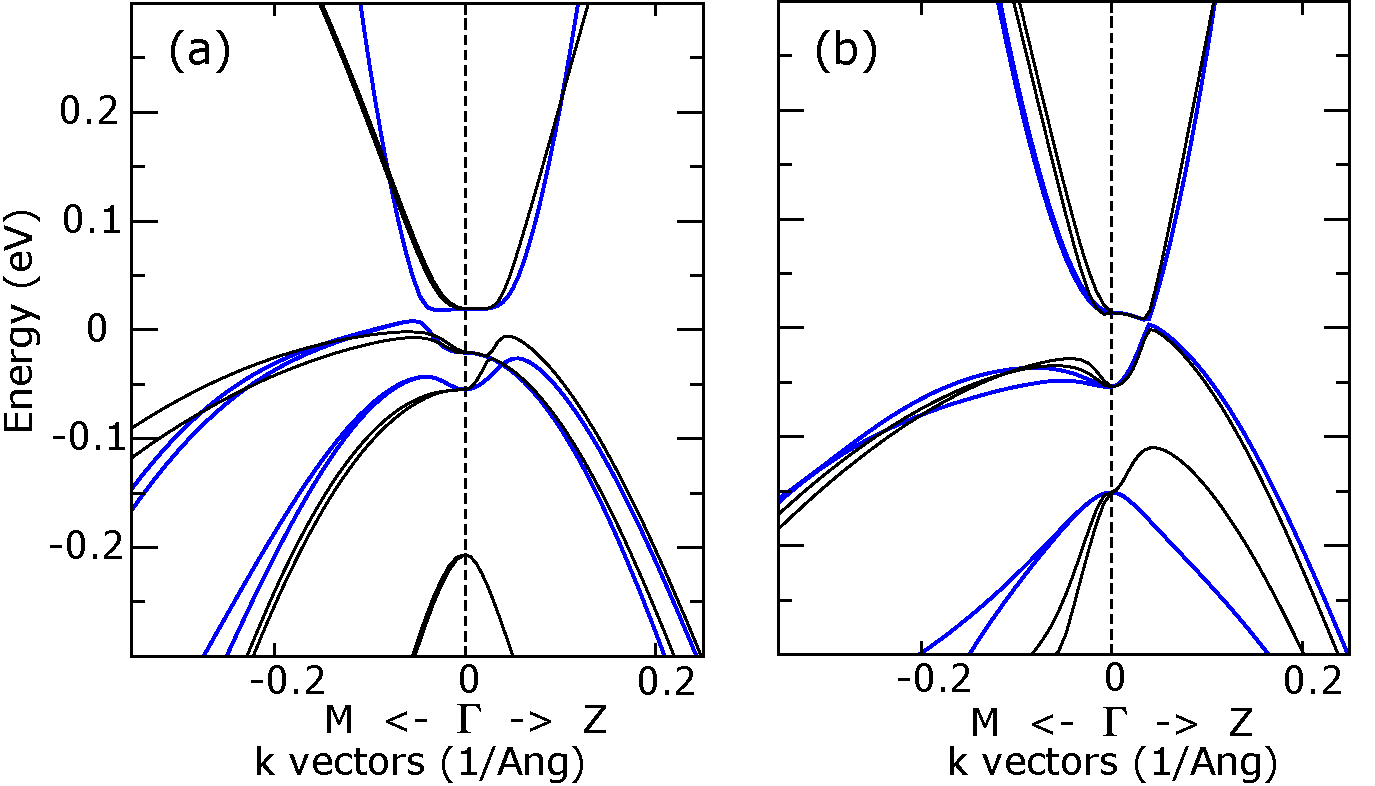
\includegraphics[height=4.3 cm]{s4-figs3.pdf}
    \bicaption{
        ~\tic~(a)和 \wsmc~(b)在$\Gamma$点附近的拟合的能带结构,拟合参数列在表格5.3中。其中黑色的线是有第一性原理计算得到的能带结构,蓝色的线是由六带模型拟合的结果。~\citep{Qians4}
    }
    {
    The fitted electronic energy bands around the $\Gamma$ point of ~\tic~(a) and ~\wsmc~(b) with fitting parameters shown in Table 5.3, where the black lines are the band structures from first-principles calculations and the blue lines are the results of the fitted effective six-band model. ~\citep{Qians4}
    }
    \label{fig:5-s3}
\end{figure}

%{\color{red}Note that the six-band model is the minimal model to describe band inversion and topological phase transation process in these candidates at $\Gamma$ point.  The $k\cdot p$ Hamiltonian was blockly built by using the invariant method. Firstly, we build the six band Luttinger model describing the $\Gamma^-_7$ and $\Gamma_8^+$ bands which label the O$_h$ group. Then by introducting the band inversion and strain term, we can reproduce the process of Weyl fermion's emergence.  Proper parameters are chosen to satisfy the condition of Weyl fermions mentioned above. }

为了获得外尔半金属相\wsm~的费米弧表面态~\citep{Wan2011,xu2011chern},我们通过引入变换: $k_{i}\rightarrow \frac{1}{L_{i}}\text{sin}[k_{i}L_{i}]$ 和 $k_{i}^2\rightarrow\frac{2}{L_{i}^2}(1-\text{cos}[k_{i}L_{i}])$,其中 $i=x,y,z$~\citep{wang2013three},将六带模型转化为四方晶格的紧束缚模型。
%k_{i}\rightarrow sin[k_{i}L_{i}], 
%k_{i}^2\rightarrow\frac{2}{L_{i}^2}(1-cos[k_{i}L_{i}]) (L_{x,y}=a,L_{z}=c).
我们使用迭代方法去获得半无限大体系的表面格林函数~\citep{WU2017,Sancho_1985}。表面格林函数的虚部是表面上的局域表面态 (LDOS) 。在半无限大(001) 和 (100) 表面计算得到的LDOS展示在图~\ref{fig:5-4}。因为外尔点恰好在电中心能级, 我们仅看到连接外尔点的费米弧态。在(001) 表面,两个同样手性的外尔点投影到同一个位置,所以每个投影点有两个弧。在 (100) 表面,投影的拓扑电荷展示在图~\ref{fig:5-4} (b) , 两个弧穿过$k_z=0$ 的线,因为它是有不平庸的$\mathbb Z_2$不变量的$k_z=0$面的边界。
\begin{figure}[!hb]
\centering
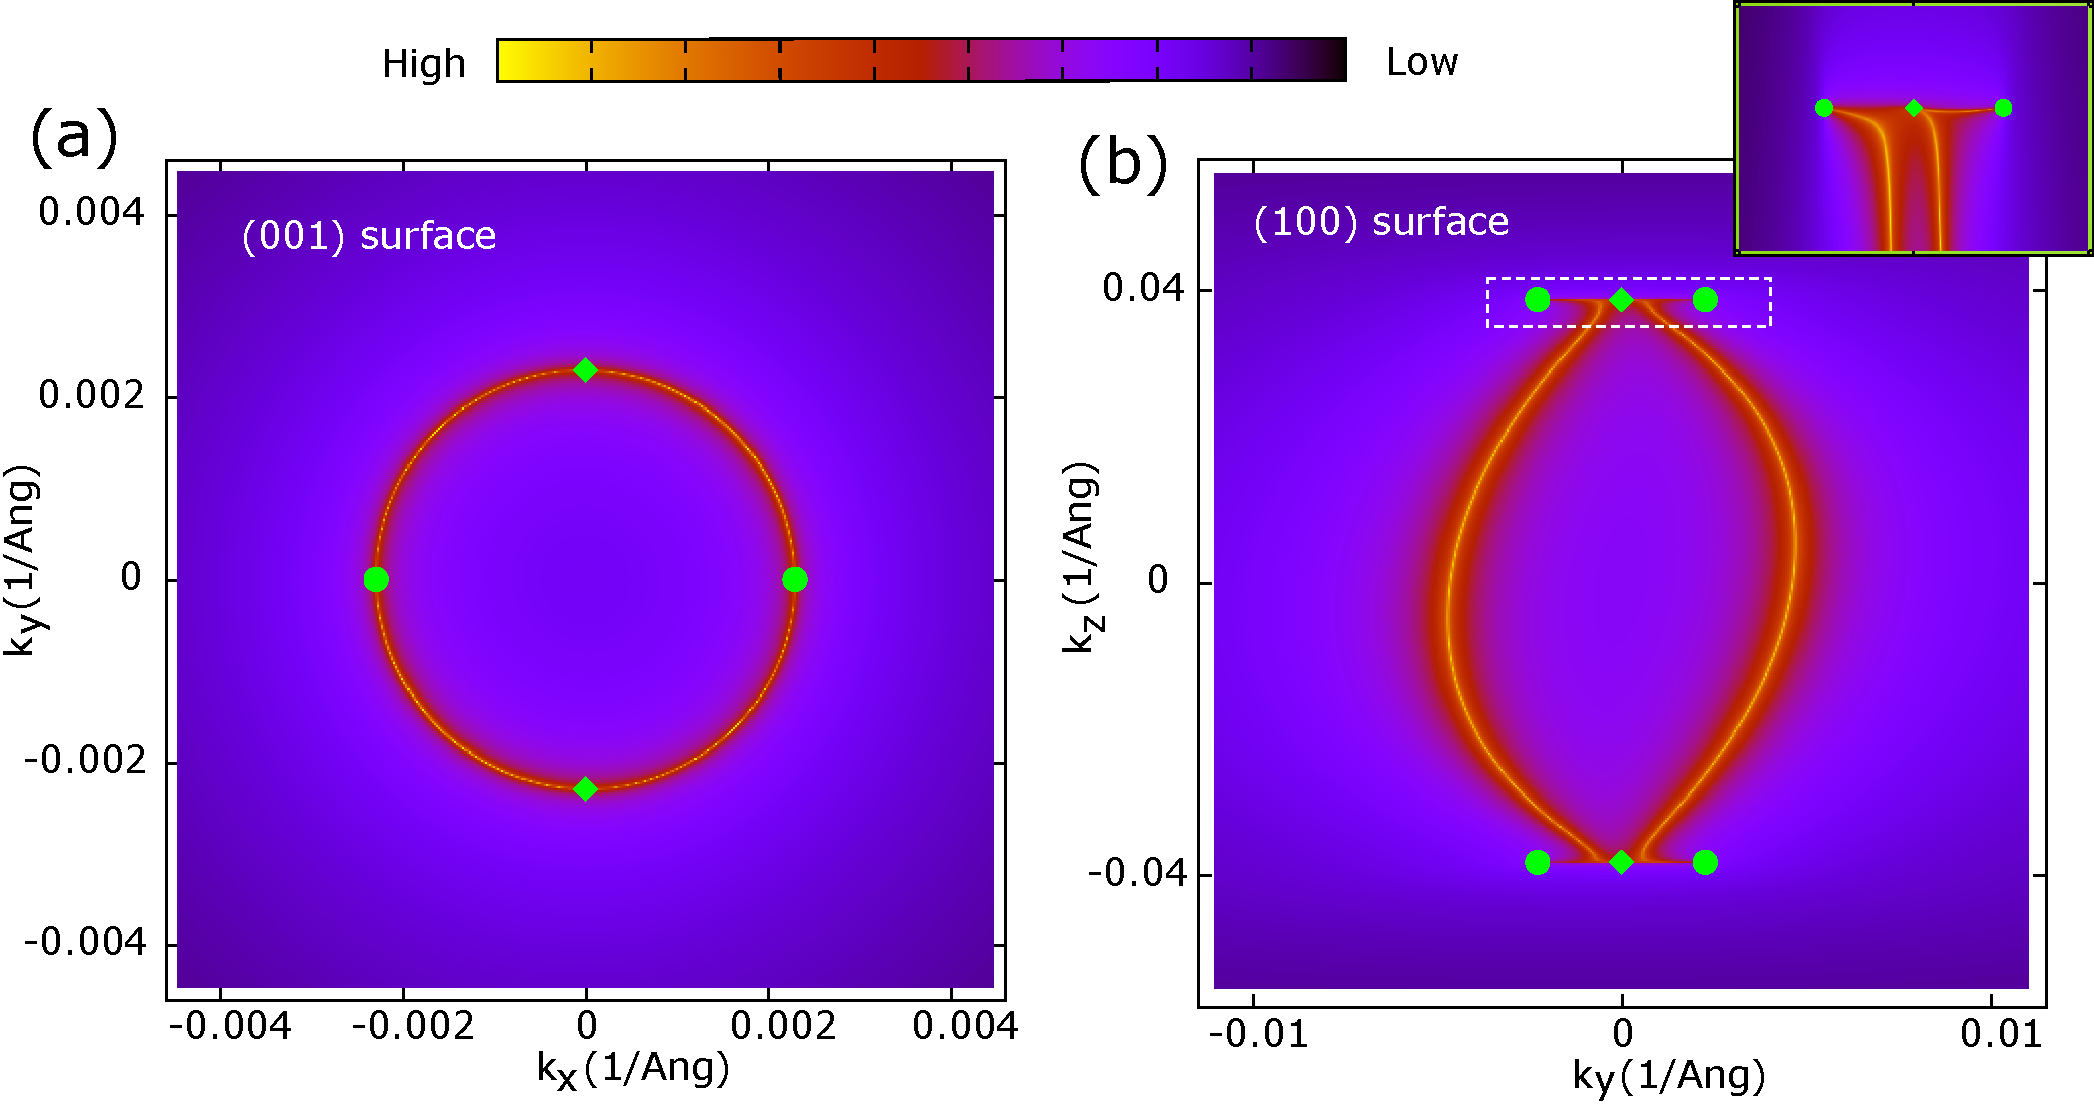
\includegraphics[width=7.5 cm]{s4-fig4.pdf}
\bicaption{
六带模型的表面费米弧。(a)(001)表面BZ的表面费米弧。(b)(100)表面BZ的表面费米弧。不同的手性的投影的外尔点用方块或者圆形表示。~\citep{Qians4}
}
{
Surface Fermi arcs of six-band model. (a) Surface Fermi arcs in the (001) surface BZ. (b) Surface Fermi arcs in the (100) surface BZ. The projected Weyl points are shown as square and circle points for different chiralities. ~\citep{Qians4}
}
\label{fig:5-4}
\end{figure}


\section{结论}
%\emph{Discussion.} --


对于外尔半金属的判据$\eta\neq z_2$可以广泛应用于其他具有$S_4$对称性的空间群。例如,我们计算了122号群的WSM CuTlSe$_2$的$z_2$不变量和$\eta$~\citep{Haijun2016}, 这个材料之前也被认为是拓扑绝缘体~\citep{Feng2011}。$\eta=1$ 和 $z_2=0$的结果表明这是个外尔半金属。另外,这个判据也可以用来理解应变的HgTe类材料的外尔相(压缩应变)和拓扑绝缘体相(拉伸应变)~\citep{HgTenc2016}。

总结一下,基于DFT计算,我们证明了先前在没有中心反演对称性但保持$S_{4z} $对称性的空间群121中预测的``TI'',实际上可以分为两种情况:$z_2=1 $ (\tii) 和$z_2=0$ (\wsm)。
这些``TIs"共同特点是时间反演的$\mathbb Z_2$不变量在$k_z=0$ 和 $k_z=\frac{\pi}{c}$的面分别为1 和 0,导致$\eta=1$。
这和绝缘相里\tii~的$S_4~z_2=1$的结论是一致的。
但是,对于``TIs"中有$S_4~z_2=0$的\wsm~实际上是外尔半金属, 这是之前没有发现的。
他们也可以作为有平庸的对称指标的拓扑材料的典例~\citep{song2017,wangprl2019}。
在 $k_{x,y}=0$面上发现四对外尔点,每个平面上四个外尔点手性相同。
我们的工作纠正了之前对这些材料已有的认识,并且预测了更多的外尔半金属候选材料,这些材料可以在之后的实验中进一步检验。
更重要的是,在时间反演不变体系中使用对称性指标和拓扑不变量方法 (即 $\eta\neq z_2$) 对于搜索外尔半金属提供了新的途径。
在此工作后期,我们对数据库中所有具有S$_4$但不具有中心反演的体系进行了高通量计算~\citep{tobedone2019},发现很多有趣外尔半金属材料。为实验和理论的研究提供了很多可选择的平台。相信我们的工作在未来将有助于大量预测外尔半金属。
\ \\


% %\newpage
% \begin{figure}[!htb]
% \centering
% 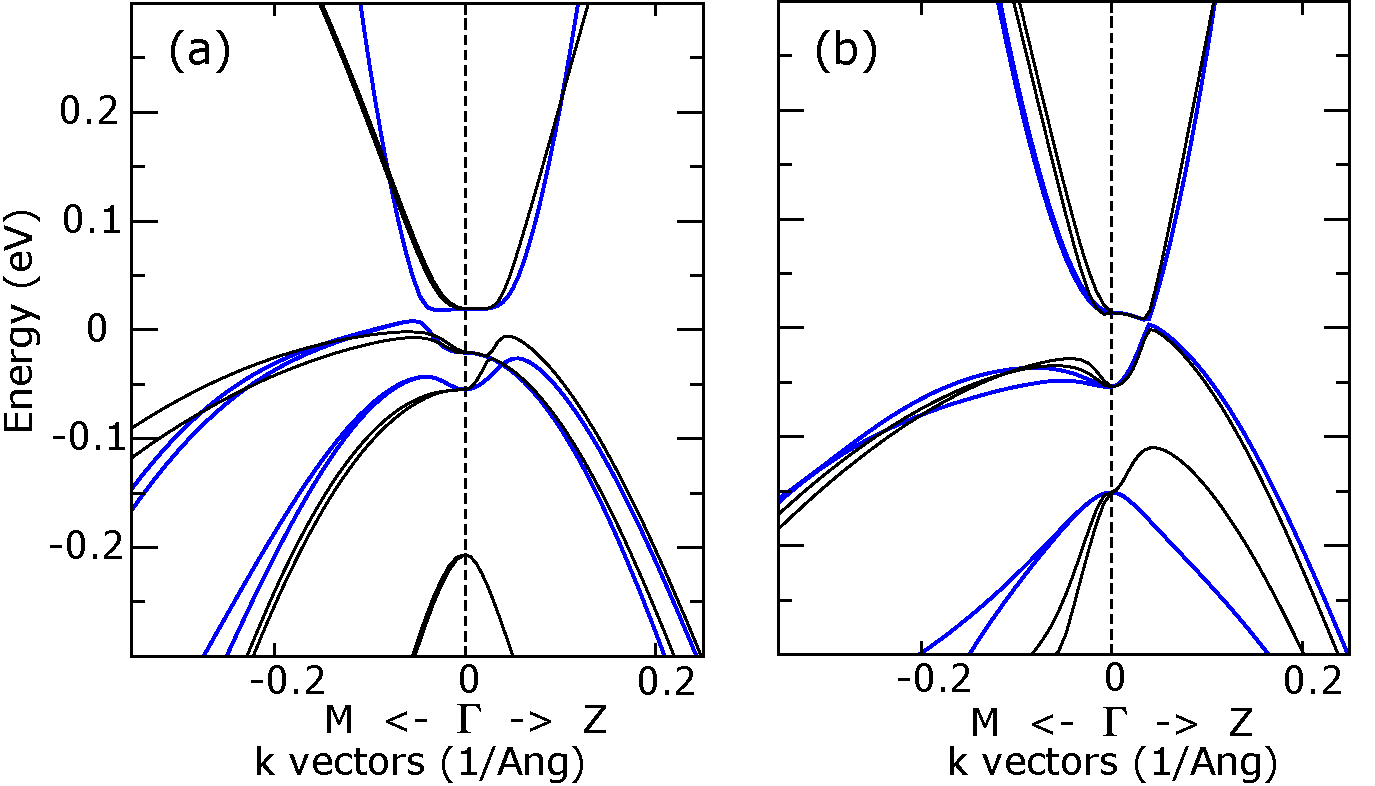
\includegraphics[height=5 cm]{s4-figs3.pdf}
% \caption{(Color online)
% The fitted electronic energy bands around the $\Gamma$ point of ~\tic~(a) and ~\wsmc~(b) with fitting parameters shown in Table I, where the black lines are the band structures from first-principles calculations and the blue lines are the results of the fitted effective six-band model.
% }
% \label{fig:5-s3}
% \end{figure}

